	En este capítulo se describe toda la información que manejará el sistema. Se describen todos los datos que serán entradas y salidas mediante la descripción de Entidades, atributos y sus relaciones. Cada entidad se representa como una clase y cada fila de la entidad le corresponde un atributo en su clase.Las relaciones entre clases se modelan utilizando conceptos como
	Participación, Composición, Agregación y Generalización. Para poder llevar a cabo la relación de atributos y clases con el negocio, se utiliza la notación UML2.0 especificada por la \href{www.omg.org}{OMG}.

%--------Modelo Estructural del Proceso de Infraestructura------------------%
\section{Modelo Estructural de Gestión de Infraestructura}
	%En la figura \ref{fig:infraestructuraDC} se muestra la estructura de información que manejará el \refElem{Calmecac} para llevar a cabo la gestión de unidades académicas, edificios y espacios.

\begin{figure}[hbtp!]
	\begin{center}
%				\fbox{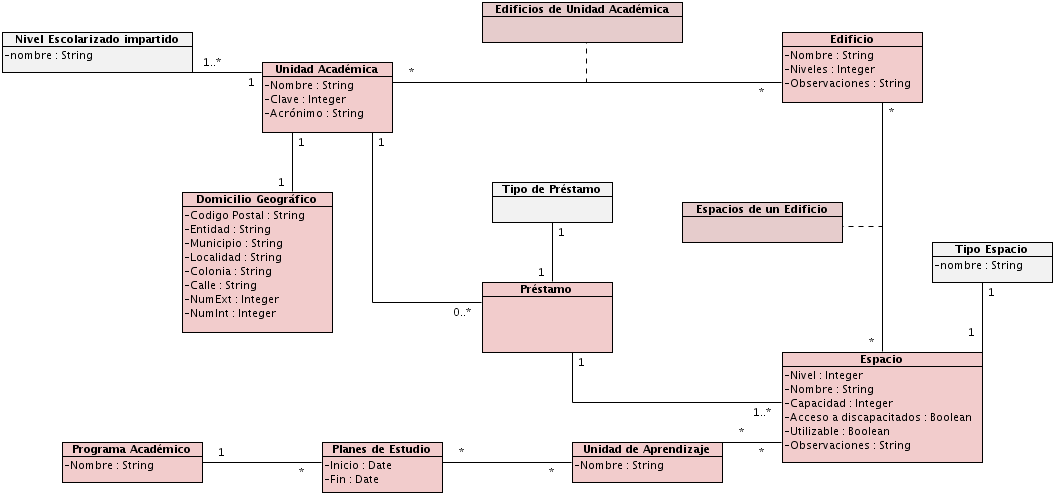
\includegraphics[width=\textwidth]{negocio/images/Modelodeinformacion_Procesodeinfraestructura_version_dos}}
%		\caption{Diagrama de Clases de Infraestructura}
%		\label{fig:infraestructuraDC}
	\end{center}
\end{figure}

%----------------------Entidades-------------------------------------------%

%=====Unidad Académica=====%
%\begin{cdtEntidad}{unidadAcademica}{Unidad Académica}
%	\brAttr{nombre}{Nombre}{Frase}{Es el nombre asignado a una unidad académica de acuerdo a los programas académicos que se imparten en ella}{\datRequerido}
%	\brAttr{clave}{Clave}{Entero}{Es la clave con la que una unidad académica puede ser identificada de otras}{\datRequerido}
%	\brAttr{acronimo}{Acrónimo}{Palabra}{Son las siglas con las que se pueden identificar las diferentes unidades académicas}{\datRequerido}
%	%----------------------------------
%	\cdtEntityRelSection
%	\brRel{\brRelAgregation}{\refElem{nivelEscolarizadoImpartido}}{Una \refElem{unidadAcademica} tiene  al menos un \refElem{nivelEscolarizadoImpartido}}
%	\brRel{\brRelComposition}{\refElem{domicilioGeografico}}{Una \refElem{unidadAcademica} reside en un \refElem{domicilioGeografico}}
%	\brRel{\brRelComposition}{\refElem{edificio}}{Una \refElem{unidadAcademica} tiene \refElem{edificio}}
%\end{cdtEntidad}



\include{negocio/informacionHorarios}
%-----------------------------Modelo Esturctural de Profesores--------------------------%
En la figura \ref{fig:infoProfesores} se puede observar la información que el \refElem{Calmecac} utilizará de acuerdo a los servicios web proporcionados por el \refElem{SIEE}.%Verificar

\begin{figure}[hbtp!]
	\begin{center}
	\fbox{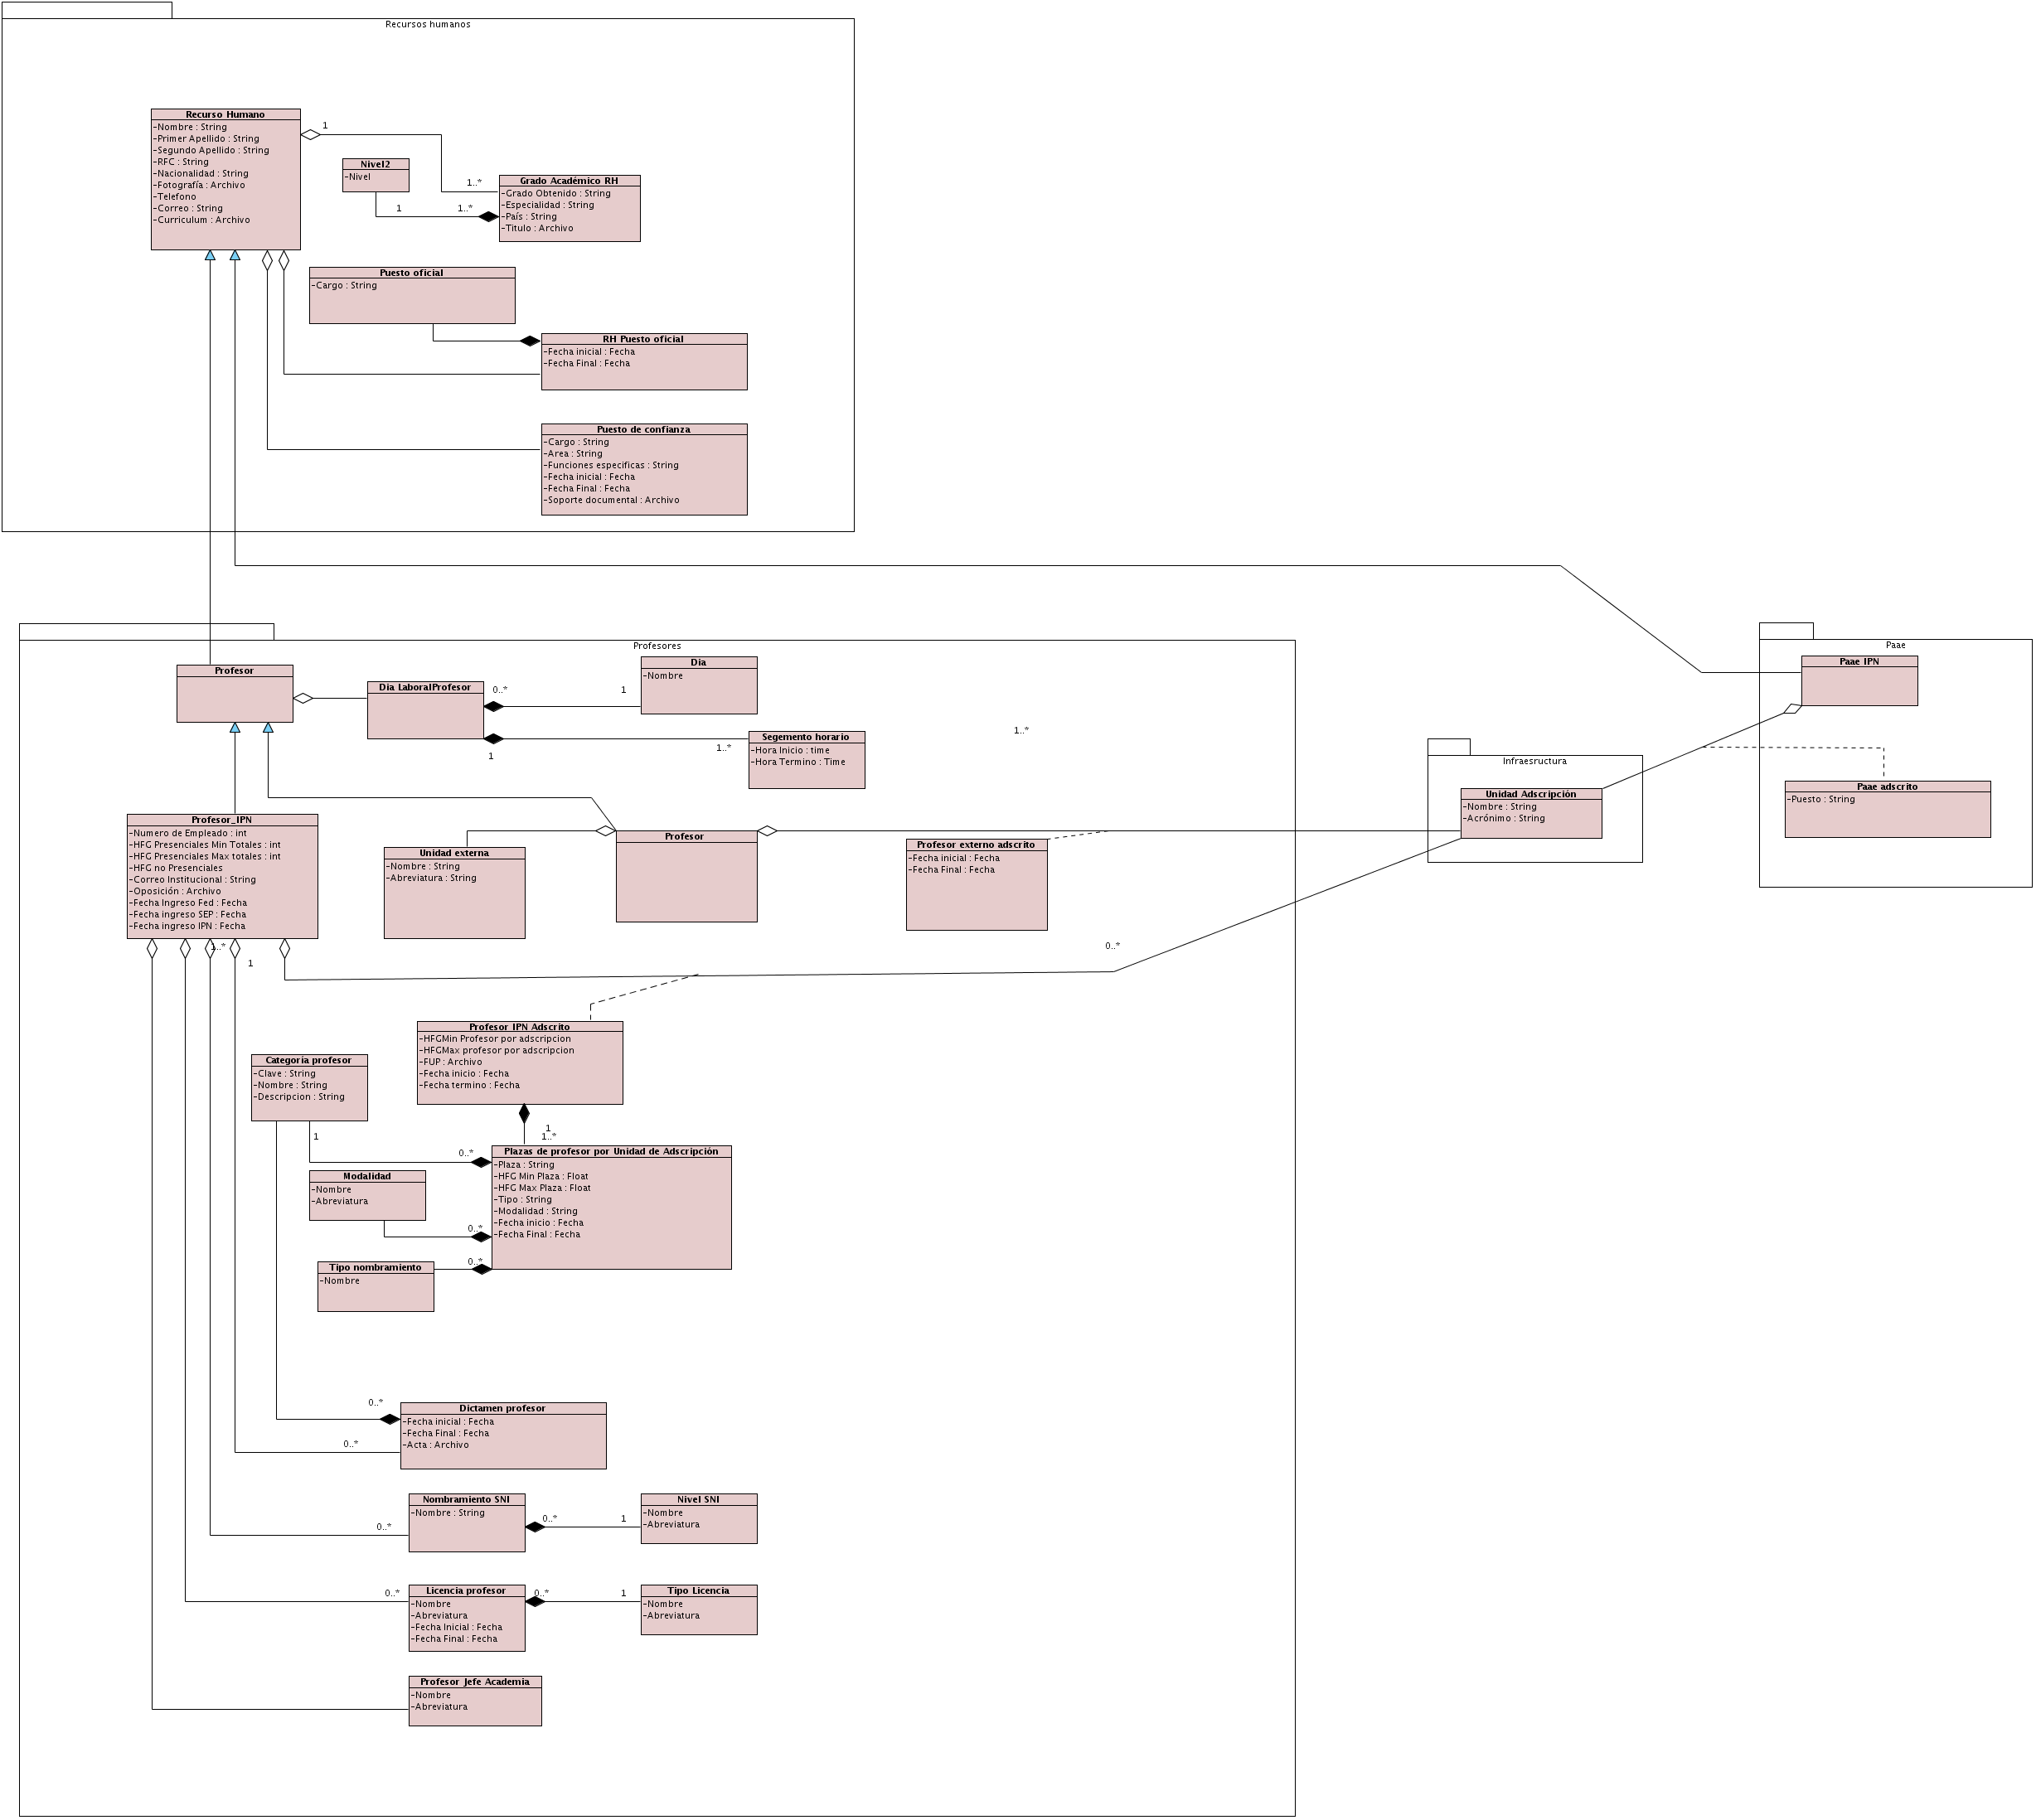
\includegraphics[width=\textwidth]{negocio/images/ModeloDeInformacion_Profesores}}
		\label{fig:infoProfesores}
		\caption{Modelo de Información de Profesores}
	\end{center}
\end{figure}

%----------------------------------Recurso Humano--------------------------------------
\begin{cdtEntidad}{RecursoHumano}{Recurso Humano}
	\brAttr{nombre}{Nombre}{Frase}{Indica el nombre del recurso humano del Instituto Politécnico Nacional.}{\datRequerido}
	\brAttr{primerApellido}{Primer apellido}{Frase}{Indica el primer apellido de un recurso humano del Instituto Politécnico Nacional.}{\datRequerido}
	\brAttr{segundoApellido}{Segundo apellido}{Frase}{Indica el segundo apellido, si lo tuviese, de un recurso humando del Instituto Politécnico Nacional.}{\datOpcional}
	\brAttr{RFC}{RFC}{Palabra}{Indica el RFC con el que el Recurso Humano se registró en el Instituto Politécnico Nacional.}{\datRequerido}
	\brAttr{CURP}{CURP}{Palabra}{Indica el CURP con el que el recurso humano se registró en el Instituto Politécnico Nacional.}{\datRequerido} %Falta en el modelo de información
	\brAttr{nacionalidad}{Nacionalidad}{Frase}{Indica al país al que pertenece el recurso humano.}{\datOpcional}
	\brAttr{fotografia}{Fotografía}{Archivo}{Es el archivo en formato JPG o PNG que contiene una fotografía del recurso humano del Instituto Politécnico Nacional.}{\datOpcional}
	\brAttr{telefono}{Teléfono}{Frase}{Contiene el número telefónico agregado o registrado con el que es posible localizar al recurso humano.}{\datOpcional}
	\brAttr{correo}{Correo electrónico}{Frase}{Contiene el correo electrónico del \refElem{RecursoHumano}.}{\datOpcional}
	\brAttr{curriculum}{Currículum}{Archivo}{Archivo que contiene los logros académicos obtenidos por el recurso humano tanto fuera como dentro del Instituto Politécnico Nacional}{\datOpcional}
	\cdtEntityRelSection
	\brRel{\brRelAgregation}{\refElem{GradoAcademico}}{Un \refElem{RecursoHumano} del Instituto ha conseguido varios o al menos un \refElem{GradoAcademico} a lo largo de su vida académica.}
	\brRel{\brRelAgregation}{\refElem{FuncionOficial}}{Un \refElem{RecursoHumano} del Instituto puede llegar a ocupar una \refElem{FuncionOficial} de una \refElem{UnidadAcademica}.Tales funciones pueden ser:
	\begin{Citemize}
		\item Director
		\item Subdirector Académico
\end{Citemize}}
	\brRel{\brRelAgregation}{\refElem{FuncionAdministrativa}}{Un \refElem{RecursoHumano} del Instituto puede llegar a ocupar una \refElem{FuncionAdministrativa}, la cual es creada de acuerdo a las necesidades particulares de cada \refElem{UnidadAcademica}.}
	\brRel{\brRelGeneralization}{\refElem{Profesor}}{Un \refElem{RecursoHumano}  es un \refElem{Profesor} o docente que imparte clases en una o varias unidades académicas\footnote{ver \refElem{UnidadAcademica}}.}
\end{cdtEntidad}

%---------------------------------------Grado Académico--------------------------------------------%
\begin{cdtEntidad}{GradoAcademico}{Grado Académico}
	\brAttr{gradoObtenido}{Grado Obtenido}{Frase}{Indica el grado que el \refElem{RecursoHumano} ha adquirido.}{\datRequerido}
	
	\brAttr{especialidad}{Especialidad}{Frase}{Indica en que área se especializó el \refElem{RecursoHumano}.}{\datRequerido}
	
	\brAttr{pais}{País}{Frase}{Indica el país en que el \refElem{RecursoHumano} obtuvo el grado académico.}{\datRequerido}
	
	\brAttr{titulo}{Título}{Archivo}{Archivo que contiene el título adquirido por el \refElem{RecursoHumano}}{\datOpcional}
	
	\cdtEntityRelSection
	
	\brRel{\brRelAgregation}{\refElem{RecursoHumano}}{Un \refElem{RecursoHumano} del Instituto ha conseguido varios o al menos un \refElem{GradoAcademico} a lo largo de su vida académica.}
	
	\brRel{\brRelAgregation}{\refElem{Nivel}}{Un \refElem{GradoAcademico} es adquirido con un cierto \refElem{Nivel} pudiendo ser entre lo más comunes:
	\begin{Citemize}
		\item Licenciatura
		\item Maestría
		\item Doctorado
\end{Citemize}}

\end{cdtEntidad}
%-------------------------------------Nível--------------------------------------------------------%

\begin{cdtEntidad}{Nivel}{Nível}
	\brAttr{nivel}{Nivel}{Frase}{Indica el nivel de un grado académico pudiendo ser:\begin{Citemize}
			\item Licenciatura
			\item Maestría
			\item Doctorado
	\end{Citemize}}{\datRequerido}

	\cdtEntityRelSection
	\brRel{\brRelAgregation}{\refElem{GradoAcademico}}{Un \refElem{GradoAcademico} es adquirido con un cierto \refElem{Nivel} pudiendo ser entre lo más comunes:
		\begin{Citemize}
			\item Licenciatura
			\item Maestría
			\item Doctorado
	\end{Citemize}}
\end{cdtEntidad}

%-----------------------------------Profesor---------------------------------------------------%

\begin{cdtEntidad}{Profesor}{Profesor}
	\cdtEntityRelSection
	\brRel{\brRelAgregation}{\refElem{DiaLaboral}}{Un \refElem{Profesor} realiza sus actividades académicas en varios días laborales\footnote{ver \refElem{DiaLaboral}}}
	\brRel{\brRelGeneralization}{\refElem{ProfesorIPN}}{Un \refElem{ProfesorIPN} es un \refElem{Profesor} en el Instituto.}
\end{cdtEntidad}


%-------------------------------------Día Laboral----------------------------------------------

\begin{cdtEntidad}{DiaLaboral}{Día Laboral}
	\cdtEntityRelSection
	\brRel{\brRelComposition}{\refElem{Dia}}{Un \refElem{DiaLaboral} se lleva a cabo en un \refElem{Dia} de la semana.}
	\brRel{\brRelComposition}{\refElem{SegmentoHorario}}{Un \refElem{DiaLaboral} se divide en segmentos de horario\footnote{ver \refElem{SegmentoHorario}}.}
\end{cdtEntidad}

%------------------------------------Día----------------------------------

\begin{cdtEntidad}{Dia}{Día}
	\brAttr{nombre}{Nombre}{Palabra}{Indica un día de la semana:\hspace{2pt}
	\begin{Citemize}
		\item Lunes
		\item Martes
		\item Miércoles 
		\item Jueves
		\item Viernes
		\item Sábado
		\item Domingo
\end{Citemize}}{\datRequerido}
\end{cdtEntidad}

%--------------------------------Profesor Ipn---------------------------------


\begin{cdtEntidad}{ProfesorIPN}{Profesor del Politécnico}
	\brAttr{numeroEmpleado}{Número de empleado}{Entero}{Es el número único asignado a cada \refElem{RecursoHumano} que está contratado por el Instituto Politécnico Nacional}{\datRequerido}
	\brAttr{HFGmin}{Horas frente a grupo mínimas}{Entero}{Es el número que representa las horas mínimas que un \refElem{ProfesorIPN} debe estar impartiendo clases en una \refElem{UnidadAcademica}}{\datRequerido}
	\brAttr{HFGmax}{Horas frente a grupo máximas}{Entero}{Es el número que representa las horas máximas que un \refElem{ProfesorIPN} debe estar impartiendo clases en una \refElem{UnidadAcademica}}{\datRequerido}
	\brAttr{HFGnoPresenciales}{Horas frente a grupo no presenciales}{Entero}{Es el número que representa las horas que el \refElem{ProfesorIPN} no imparte clases.}{\datRequerido}
	\brAttr{correo}{Correo electrónico Institucional}{Frase}{Contiene el correo electrónico Institucional asignado al recurso humando cuando ingresó como parte de la comunidad Politécnica.}{\datOpcional}
	\brAttr{oposicion}{Oposición}{Archivo}{Es el archivo que contiene el examen de oposición que el \refElem{ProfesrIPN} realizó para poder impartir clases en el Instituto Politécnico Nacional}{\datOpcional}
	\brAttr{fechaIngreso}{Fecha de Ingreso}{Fecha}{Fecha en la que el \refElem{ProfesorIPN} }{\datOpcional}
	\brAttr{fechaIngresosEP}{Fecha de Ingreso a la SEP}{Fecha}{Fecha en la que el \refElem{ProfesorIPN} ingresó a la SEP}{\datOpcional}
	\brAttr{fechaIngresoIPN}{Fecha de Ingreso al IPN}{Fecha}{Fecha en la que el \refElem{ProfesorIPN} ingresó al Instituto}{\datOpcional}
\end{cdtEntidad}
\include{negocio/informacion-Alumno}
\include{negocio/informacion-EE}
\include{negocio/informacion-SD}

